% !TeX spellcheck = en_US

\chapter{Extending minimal DFAs} \label{ch:3}

We firstly define a formal problem for extending a minimal DFA $A_{sol}$ to a task DFA $A_{task}$ based on our requirements analysis (see~\ref{ch:1:determined-requirements}):
\begin{definition}[ExtendMinimalDFA] $ $ \\
	$ $ \vspace{-0.4cm} \\
	\noindent $\underline{\emph{Given:}}$
	\vspace{-0.5cm}
	\begin{align*}
	A_{sol} = (Q, \Sigma, \delta, s, F) \in \mathcal{A}_{min}\ \ \ & \emph{solution DFA} \\
	\mathfrak{r} \in \mathbb{N}\ \ \ & \emph{number of redundant states} \\
	\mathfrak{u} \in \mathbb{N}\ \ \ & \emph{number of unreachable states} \\
	p \in \{0,1\}\ \ \ & \emph{planarity-bit} \\
	c \in \{0,1\}\ \ \ & \emph{completeness-bit}
	\end{align*}
	\noindent $\underline{\emph{Task:}}$ \emph{Compute, if it exists, a task DFA $A_{task}$ with}
	\begin{itemize}
		\item $Q_{task} = Q_{sol} \cup \{ r_1, \ldots, r_\mathfrak{r}, u_1, \ldots, u_\mathfrak{u} \}$
		\item $r_1, \ldots, r_\mathfrak{r}$ \emph{redundant}
		\item $u_1, \ldots, u_\mathfrak{u}$ \emph{unreachable}
		\item $\Sigma_{task} = \Sigma_{sol}$, $s_{task} = s_{sol}$, $F_{task} \subseteq F_{sol}$
		\item $A_{task}$ \emph{being planar iff} $p = 1$
		\item $A_{task}$ \emph{being complete iff} $c = 1$
		\item $A_{sol}$ \emph{being isomorph to} $\MinAlg(A_{task})$
	\end{itemize}
\end{definition}
\noindent In order to fulfill these requirements we will deduce for both kinds of states how they may be added by examining their desired properties. We will show for the action of adding redundant states, that this does not change a DFAs $\mmD$-value.

\section{Creating equivalent state pairs}

Step 3 and 4 of the minimization algorithm are concerned with detection and elimination of equivalent state pairs. We now want to add states $r_1,\ldots,r_\mathfrak{r}$ to a DFA $A_{sol}$, gaining $A_{re}$ with $Q_{re} = Q_{sol} \cup \{r_1,\ldots,r_\mathfrak{r}\}$, such that each of these states is equivalent to a state in $A_{re}$. Note that, for reasons of clarity, we are going to abbreviate from now on $A_{re} = A$, $Q_{re} = Q$, $\sim_{A_{re}} = \sim_A$ etc.

%At this point we notice, that $A_{sol}$ is isomorph to the $\sim$-equivalence automaton (see def.~\ref{ch:1:sim-eq-dfa}). We can think 

Consider the properties $r_1,\ldots,r_\mathfrak{r}$ must have. They are equivalent to states $o_1,\ldots,o_\mathfrak{r}$ of $A$.
\[
\exists r_1,\ldots,r_\mathfrak{r} \in Q\colon\ \exists o_1,\ldots,o_\mathfrak{r} \in Q\colon\ \forall i \in [1,\mathfrak{r}] \colon\ r_i \sim_A o_i
\]
But we know also and in particular, that each of them is equivalent a state $e$ of $A_{sol}$.
\[
	\exists r_1,\ldots,r_\mathfrak{r} \in Q\colon\ \forall i \in [1,\mathfrak{r}] \colon\ \exists e \in Q_{sol}\colon\ r_i \sim_A e
\]
In our algorithm, we will choose the state $e$ for each state we add.

\subsection{Adding outgoing transitions}

Regarding the outgoing transitions of any $r_i$ equivalent to a state $e$, we are directly restricted by the relationship $\forall \sigma \in \Sigma \colon [\delta(r_i, \sigma)]_{\sim_A} = [\delta(e, \sigma)]_{\sim_A}$. Thus, when adding some $r_i$, we have to choose for each symbol $\sigma \in \Sigma$ at exactly one transition (completeness requirement for $A$) from the following set:
\[
	O_{e,\sigma} = \{\ ((r_i, \sigma), q)\ |\ q \in [\delta(e, \sigma)]_{\sim_A}\ \}
\]
Since the solution DFA is complete and since every here added state gets a transition for every alphabet symbol, we know that every $O_{e,\sigma} \neq \emptyset$.

\gregor{Why does this not affect the eq. class of any other state?}

\subsection{Adding ingoing transitions}

First of all, we know, that $r_i$ is reachable, since every state of $A$ must be reachable, so we need to give $r_i$ at least one ingoing transition. Doing this, we have to ensure, that any state $q$, that gets such an outgoing transition to $r_i$ remains in its $\sim$-equivalence class.
	
Thus a fitting state $q$ has to have a transition to some state in $[r_i]_{\sim_A} = [e]_{\sim_A}$ already. So, given a state $q$ with $\delta(q, \sigma) = p$ and $p \in [e]_{\sim_A}$, we can set $\delta(q, \sigma) = r_i$ and thus ``steal'' $q$ its ingoing transition.

We see here, that $q$ must have at least $2$ ingoing transitions, else it would become unreachable. Thus we summarize:
\[
    I_e = \{\ ((q, \sigma), p)\ |\ \delta(q, \sigma) = p \land p \in [e] \land d^-(p) \geq 2\ \}
\]
Choose at least one $((q, \sigma), p) \in I_e$, remove $((q, \sigma), p)$ from $\delta$ and add $((q, \sigma), r_i)$. 

These finding lead us to a general requirement regarding the choice of a state $e$ for an $r_i$: The equivalence class of any $e$ has to contain at least one state with at least $2$ ingoing transitions (see fig.~\ref{fig:dfa_add_redundant_states}). We establish the following notion to pin down this restriction:
\[
	duplicatable(q) \Leftrightarrow_{def} (\exists p \in [q]_{\sim_A}\colon |d^-(p)| \geq 2)
\]
The number of duplicatable states in any accessible DFA $A$ is $0$ for $|\Sigma| \leq 1$ (due to the restriction $|d^-(p)| \geq 2$) and greater than $0$ for $|\Sigma| > 1$ due to the pigeonhole principle: An accessible complete DFA has $|Q||\Sigma|$ transitions which have to be spread across $|Q|$ states.
\begin{figure}
	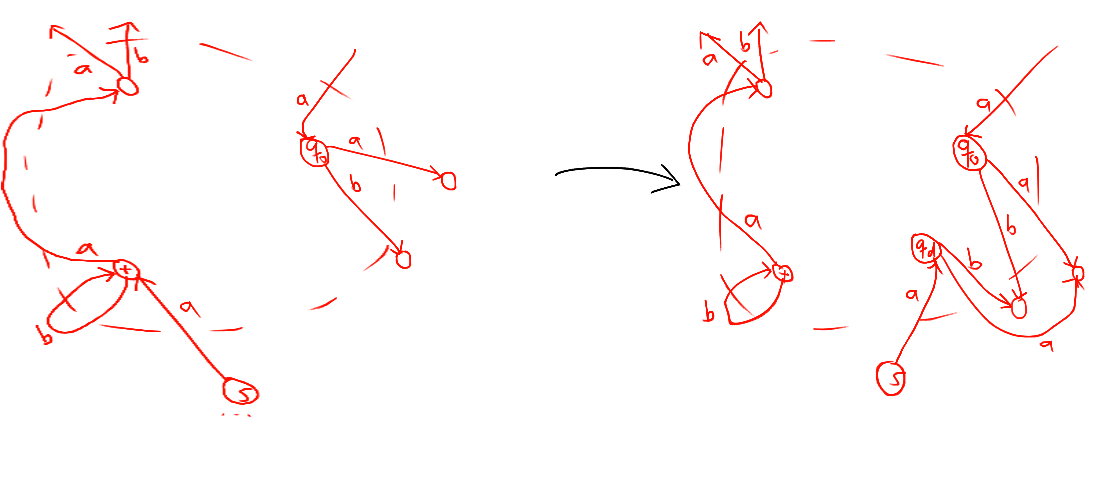
\includegraphics[width=\linewidth]{images/dfa_add_redundant_states.png}
	\caption{If an equivalence class (here denoted by the states in the dashed area) contains a state with 2 or more ingoing transitions (in this case $p$), then a state equivalent to any of the classes states may be added. Here $r$ is equivalent to $o$ and is ``stealing'' the ingoing transition $\delta(q, a)$ from $p$.}
	\label{fig:dfa_add_redundant_states}
\end{figure}

\subsection{The algorithm}

\vspace{0.2cm}
\begin{spacing}{1}
\begin{algorithmic}[1]
	\Function{AddRedundantStates}{$A, \mathfrak{r}$}
    \State $Q \gets Q_{sol}$
    \State $\delta \gets \delta_{sol}$
    \State $F \gets F_{sol}$
	\State $K \gets \{\ \{q\}\ |\ q \in Q\ \}$ \Comment{tracks the equivalence classes of $A$}
	\State $k(q) = C$ such that $q \in C$ and $C \in K$ \Comment{returns the equivalence class to $q$}
	\State $in(q) = |d^-(q)|$ for all $q \in Q$ \Comment{tracks the number of ingoing t.}
	
    \For {$i$ \textbf{in} $[1,\mathfrak{r}]$}
		\For {$q$ \textbf{in} $Q$} \Comment{find a duplicatable state $e$}
			\If {$in(q) \geq 2$}
				\State $e \gets$ random chosen state from $k(q)$
				\State \textbf{break}
			\EndIf
		\EndFor
		
        \State Add $r_i$ to $Q$ \Comment{create to $e$ equivalent state $r_i$}
		\State Add $r_i$ to $k(e)$
		
		\For {$\sigma$ \textbf{in} $\Sigma$} \Comment{add $d^+(r_i)$}
			\State $\delta(r_i, \sigma) =$ random chosen state from $k(\delta(e, \sigma))$
		\EndFor
		
		\State $P \gets \{\ ((s, \sigma), t) \in \delta\ |\ t \in k(e),\ in(t) \geq 2\ \}$ \Comment{add $d^-(r_i)$}
		\State $C \gets$ random nonempty subset of $P$
		\For {$((s, \sigma), t)$ \textbf{in} $C$}
			\State $in(t) \gets in(t) - 1$
			\State $in(r_i) \gets 1$
            \State $\delta(s, \sigma) = r_i$
		\EndFor
	\EndFor
    \State \Return $(Q, \Sigma_{sol}, \delta, s_{sol}, F)$
	\EndFunction
\end{algorithmic}
\end{spacing}
\vspace{0.2cm}

\subsection{Creating equivalent state pairs does not change $\mmD$} \label{ch:3:sec-D-proof}

To prove this statement, we will prove two minor propositions first. In this context we will call a word $w$ \emph{distinguishing word of $p,q$}, iff $distinguishes(w, q_0, q_1)$ whereas $distinguishes_A(w, q_0, q_1) \Leftrightarrow (\delta^*(p,w) \in F \Leftrightarrow \delta^*(q,w) \notin F)$.

\begin{lemma}[Semantics of $(p,q) \in m(n)$] \label{ch:3:semantics-of-m(n)}
    In the context of \CompDist\ the following is true:
    \[
        (p,q) \in m(n) \Longleftrightarrow \exists w\in\Sigma^*\colon (|w| = n\ \land distinguishes_A(w, p, q))
    \]
\end{lemma}

\begin{proof}
	See TI-Lecture ch. 4 ``Minimization'' p. 18.
\end{proof}

\begin{lemma}[Semantics of $\mmD(A) = n$] \label{ch:3:semantics-of-D(A)}
	\begin{multline*}
		\mmD(A) =\ n \Rightarrow \\
		n = \max_{n \in \mathbb{N}}\ \ \exists p, q \in Q\ \ \exists w \in \Sigma^* \colon \hspace{3cm} \\
		(|w| = n - 1\ \land distinguishes_A(w, p, q))
	\end{multline*}
\end{lemma}

\begin{proof}
		Via direct proof. Assume $m$-\CompDist(A) has done $n$ iterations (so $\mmD(A) = n$). We then know, that
		\begin{enumerate}
			\item $\forall i \in [0,n-1]\colon m(i) \neq \emptyset$
			\item $\forall i \geq n\colon m(n)= \emptyset$ \gregor{fix this}
		\end{enumerate}
		$m$-\CompDist(A) terminates iff $m(i) = \emptyset$. If the first point would not hold, then the algorithm would have stopped before.
		
		Since the algorithm did $n$ iterations, the internal variable $i$ must be $n$ at the end of the last iteration. The terminating condition is $m(i) \neq \emptyset$; thus follows the second point.
        
        We prove that then there exists a distinguishing word of length $n-1$, but the existence of a longer word leads to a contradiction. Recall lemma~\ref{ch:3:semantics-of-m(n)}:
        \[
            (p,q) \in m(n) \Longleftrightarrow \exists w\in\Sigma^*\colon (|w| = n\ \land distinguishes(w, p, q))
        \]
	
		% a possible word per definition of D(A), m(i) and lemma
		
		\noindent Following this lemma and point 1, we can deduce that there exists at least one distinguishing word $w$ with $|w| = n-1$ for some $p,q \in Q$.
		
		% There is no word longer than that
		
		There cannot be any distinguishing word $w'$ with $|w'| = k > n-1$ for any two states $p',q'\in Q$ fulfilling this property. Following the lemma again, $m(k), k > n-1$ would be non-empty, which is contradictory to point 2.
\end{proof}

\begin{theorem}[]
	Creating equivalent state pairs in a minimal DFA $A$ does not increase the number of iterations when the \CompDist-algorithm is applied on it.
\end{theorem}

\begin{proof}
	Proof per contradiction.
	
	\noindent Let us assume there were $\mathfrak{r}$ states $r_1, \ldots, r_\mathfrak{r}$ added to the given minimal DFA $A = (Q, \Sigma, \delta, s, F)$ resulting in a DFA $A' = (Q', \Sigma, \delta', s, F')$ such that $\mmD(A) < \mmD(A')$. Concerning $A'$ we can observe the following:
	\begin{itemize}
		\item $Q' = Q \cup \{ r_1, \ldots, r_\mathfrak{r} \}$
		\item W.l.o.g. $\forall i \in [1,\mathfrak{r}] \colon\ \exists e \in Q_{sol}\colon\ r_i \sim_{A'} e$
	\end{itemize}
	Let us furthermore say that $\mmD(A) = i$ and $\mmD(A') = j$, so $i < j$. Recall now lemma~\ref{ch:3:semantics-of-D(A)}:
	\begin{multline*}
        \mmD(A) =\ n \Rightarrow \\
        n = \max_{n \in \mathbb{N}}\ \ \exists p, q \in Q\ \ \exists w \in \Sigma^* \colon \hspace{3cm} \\
        (|w| = n - 1\ \land distinguishes_A(w, p, q))
    \end{multline*}
	According to this lemma there are words $w$ with $|w| = i - 1$ and $w'$ with $|w'| = j - 1$ which are the longest distinguishing words for some states of $A$ resp.\ some states $q',p'$ of $A'$.
    
    Recall now
    \begin{lemma}\label{ch:3:lem:disting-trans}
        \[
        distinguishes_A(w, p, q) \land q \sim_A q' \Rightarrow distinguishes_A(w, p, q')
        \]
    \end{lemma}
    \begin{description}
        \item[Case 1 - $p',q'$ both in $Q$] $ $
        
        Since the longest distinguishing word any state pair $p,q \in Q$ can have is guaranteed shorter than $w'$, we know that no $p,q \in Q$ can have $w'$ as distinguishing word. \hfill\lightning
        
        \item[Case 2 - one of $p',q'$ in $Q$, one in $Q'\setminus Q$] $ $
        
        W.l.o.g. $p' \in Q, q' \in Q'\setminus Q$. We then know, that $q' \in \{r_1, \ldots, r_\mathfrak{r}\}$. This implies that $q' \sim_{A'} e$ for an $e \in Q$. By lemma~\ref{ch:3:lem:disting-trans} $distinguishes_A(w', p', e)$. But then two states from $Q$ would have $w'$ as distinguishing word which is contradictory, see above. \hfill\lightning
        
        \item[Case 3 - $p',q'$ both in $Q'\setminus Q$] $ $
        
        Analogue to case 2, we can find states $e_1, e_2 \in Q$ equivalent to $p',q'$. Then again two states from $Q$ would have $w'$ as distinguishing word. \hfill\lightning
    \end{description}
    Thus we have led our assumption to contradiction in every case, which finishes the proof.
	
%	Let us split $w'$ as $w' = u'v'$ such that $|v'| = i$, which is exactly one symbol longer than $w$. We can formulate the following statement:
%    
%    The word $v'$ is a distinguishing word for some $p,q \in Q'$.
%	\begin{equation}
%    	\text{There must exist }p, q \in Q'\text{ such that }\delta'^*(p,v) \in F' \Leftrightarrow \delta'^*(q,v) \notin F'.
%	\end{equation}
%	\gregor{hidden formulations here}
%	%There must exist $p, q \in Q'$ such that $\delta'^*(p,v) \in F' \Leftrightarrow \delta'^*(q,v) \notin F'$.
%	
%	%So there exists a minimization word $v$ in $A'$, which is exactly one symbol longer than the longest minimization word of $A$. This word has length $i$ and is detected at minimization depth $i + 1$.
%	
%	\noindent We can therefore state, that $\neg(p \in Q \land q \in Q)$, because else $\mmD(A)$ would be higher than $i$ too.  So at least one of $p,q$ must be in $Q' \setminus Q$ which is exactly $\{ q_r^1, \ldots, q_r^n \}$.
%	
%	\begin{itemize}
%		\item Every $q_r^k$ is $d_{A'}$-equivalent to a $q \in Q$
%		\item In every case, $p,q$ can be $d_{A'}$-exchanged s.t. $p,q \in Q$
%		\item But that's contradictory to $\mmD(A) = n$, because $p,q$ belong to a minimization word $w = n-1$
%	\end{itemize}
		
%	Since $q_r$ is the only new state in $A'$ compared to $A$, we can conclude that at least one of both states must be $q_r$. Since $p = q_r = q$ is contradictory (\gregor{why?}), we can conclude that exactly one of both states $p, q$ is $q_r$ and that the other one is not.
%	
%	W.l.o.g.\ we say $q = q_r$ and $p \in Q' \setminus \{q_r\} = Q$ and reformulate our statement above:
%	\begin{equation}
%	\text{There must exist a }p \in Q\text{ such that }\delta'^*(p,v) \in F' \Leftrightarrow \delta'^*(q_r,v) \notin F'.
%	\end{equation}
%	\gregor{hidden formulations here}
%	
%	%Therefore we know there exists a state $p \in Q$ such that $\exists v \in \Sigma^*$, $|v| = i$ and $\delta'^*(p,v) \in F' \Leftrightarrow \delta'^*(q_r,v) \notin F'$
%	
%	Since for $q_o \in Q$ the relation $d_{A'}(q_o, q_r)$ is given, we know per definition of $d_{A'}$ that $\forall z\in\Sigma'^*\colon \delta'^*(q_o,z) \in F \Leftrightarrow \delta'^*(q_r,z) \in F$.
%	
%	This implies in combination with statement 2.2, that for $p,q_o$ the word $v\in\Sigma'^*$ would fulfill $\delta'^*(p,v) \in F' \Leftrightarrow \delta'^*(q_o,v) \notin F'$ too. But this is contradictory to $p,q \notin Q$.
\end{proof}

\gregor{Old proof for one $q_r$}
%\begin{proof}
%	\begin{description}
%		\item
%		
%		Proof per contradiction.
%		
%		Let's assume adding a redundant state $q_r$ to a given automaton $A = (Q, \Sigma, \delta, s, F)$ results in an automaton $A' = (Q', \Sigma, \delta', s, F')$ whereas $\mmD(A) < \mmD(A')$.
%		
%		Concerning $A'$ we can say the following:
%		\begin{itemize}
%			\item $Q' = Q \cup \{ q_r \}$
%			%			\item $\delta \subseteq \delta'$
%			%			\item $F \subseteq F'$
%			\item $\exists q_o \in Q \colon\ \sim_A'(q_o, q_r)$
%		\end{itemize}
%		Let us furthermore say that $\mmD(A) = i$ and $\mmD(A') = j$. Recall now lemma~\ref{ch:3:semantics-of-D(A)}:
%		\begin{multline*}
%			\mmD(A) =\ n \Rightarrow \\
%			n = \max_{n \in \mathbb{N}}\ \ \exists p, q \in Q\ \ \exists w \in \Sigma^* \colon |w| = n - 1\ \land \\
%			(\delta^*(p,w) \in F \Leftrightarrow \delta^*(q,w) \notin F)
%		\end{multline*}
%		According to this lemma there must be a pair $s, t \in Q'$ to which exists a word $w \in \Sigma'^*$, $|w| = j - 1$, such that $\delta'^*(s,w) \in F' \Leftrightarrow \delta'^*(t,w) \notin F'$.
%		
%		Let us split $w$ as $w = uv$, whereas $u,v \in\Sigma'^*$ and $|v| = i$, which is exactly one symbol longer than the longest minimization word of $A$. We can formulate the following statement:
%		\begin{equation}
%		\text{There must exist }p, q \in Q'\text{ such that }\delta'^*(p,v) \in F' \Leftrightarrow \delta'^*(q,v) \notin F'.
%		\end{equation}
%		\gregor{hidden formulations here}
%		%There must exist $p, q \in Q'$ such that $\delta'^*(p,v) \in F' \Leftrightarrow \delta'^*(q,v) \notin F'$.
%		
%		%So there exists a minimization word $v$ in $A'$, which is exactly one symbol longer than the longest minimization word of $A$. This word has length $i$ and is detected at minimization depth $i + 1$.
%		
%		We can therefore state, that $\neg(p \in Q \land q \in Q)$, because else $\mmD(A)$ would be higher than $i$ too. 
%		
%		Since $q_r$ is the only new state in $A'$ compared to $A$, we can conclude that at least one of both states must be $q_r$. Since $p = q_r = q$ is contradictory (\gregor{why?}), we can conclude that exactly one of both states $p, q$ is $q_r$ and that the other one is not.
%		
%		W.l.o.g.\ we say $q = q_r$ and $p \in Q' \setminus \{q_r\} = Q$ and reformulate our statement above:
%		\begin{equation}
%		\text{There must exist a }p \in Q\text{ such that }\delta'^*(p,v) \in F' \Leftrightarrow \delta'^*(q_r,v) \notin F'.
%		\end{equation}
%		\gregor{hidden formulations here}
%		
%		%Therefore we know there exists a state $p \in Q$ such that $\exists v \in \Sigma^*$, $|v| = i$ and $\delta'^*(p,v) \in F' \Leftrightarrow \delta'^*(q_r,v) \notin F'$
%		
%		Since for $q_o \in Q$ the relation $d_{A'}(q_o, q_r)$ is given, we know per definition of $d_{A'}$ that $\forall z\in\Sigma'^*\colon \delta'^*(q_o,z) \in F \Leftrightarrow \delta'^*(q_r,z) \in F$.
%		
%		This implies in combination with statement 2.2, that for $p,q_o$ the word $v\in\Sigma'^*$ would fulfill $\delta'^*(p,v) \in F' \Leftrightarrow \delta'^*(q_o,v) \notin F'$ too. But this is contradictory to $p,q \notin Q$.
%		
%		\gregor{hidden lemma here}
%		
%		%		\begin{lemma}
%		%			\begin{multline*}
%		%				\mmD(A) =\ n \Leftrightarrow \\
%		%				n = \max_{n \in \mathbb{N}}\ \ \exists p, q \in Q\ \ \exists w \in \Sigma^* \colon \\
%		%				|w| = n - 1 \land (\delta^*(p,w) \in F \Leftrightarrow \delta^*(q,w) \notin F)
%		%			\end{multline*}
%		%		\end{lemma}
%	\end{description}
%\end{proof}

\section{Adding unreachable states}

From step 1 of the minimization algorithm we can deduce how to add unreachable states. These can easily be added to a DFA by adding non-start states with no ingoing transitions (see def.~\ref{ch:1:unreachable-states}). Number and nature of outgoing transitions may be arbitrary.

\vspace{0.2cm}
\begin{algorithmic}[1]
	\Function{AddUnreachableStates\ }{$A, u$}
	\For {$u$ \textbf{times}}
		\State $q \gets \max Q + 1$
		\State $Q \gets Q \cup \{ q \}$
		\State $R \gets$ random chosen sample of $|\Sigma|$ states from $Q \setminus \{q\}$
		\For {$\sigma$ \textbf{in} $\Sigma$}
			\State $q' \in R$
			\State $R \gets R \setminus \{q'\}$
			\State $\delta \gets \delta \cup \{ ((q, \sigma), q') \}$
		\EndFor
	\EndFor
	\State \Return $A$
	\EndFunction
\end{algorithmic}
\vspace{0.2cm}

%\noindent We have to ensure, that this algorithm does not induce changes in the language.
%\begin{lemma}
%	Adding unreachable states to a DFA does not change its language.
%\end{lemma}
%\begin{proof}
%	{\setlength{\parindent}{0pt}
%		Remember that the language of a DFA $A = (Q, \Sigma, \delta, s, F)$ is defined as $L(A) = \{\ w\ |\ w \in \Sigma^* \ \}$. For any unreachable state $q$ there exists no word $v \in \Sigma^*$ such that $\delta^*(s,v) = q$. Thus such a state cannot be the cause for any word to be in $L(A)$.
%	}
%\end{proof}
%
%\noindent The question whether adding unreachable states to a DFA changes $\mmD$-value is irrelevant. This is because in the context of the minimization algorithm, unreachable states are eliminated before the \CompDist-algorithm is applied on the task DFA.
